\documentclass[12pt,a4paper]{article}
\usepackage[utf8]{inputenc}
\usepackage[T1]{fontenc}
\usepackage[francais]{babel}
\usepackage{amsmath,empheq}
\usepackage{amsfonts}
\usepackage{amssymb}
\usepackage{graphicx}
\usepackage[top=2.00cm]{geometry}
\usepackage{titlesec}
\usepackage{multicol}
\usepackage{tikz,tkz-tab}
\usepackage{enumitem}
\usepackage{bigcenter}
%%modif des titres de section diminuer la taille
\graphicspath{{images/}}
\renewcommand{\thesection}{\Roman{section}}
\titleformat{\section}
{\normalfont\bfseries\Large\scshape}{\thesection}{1em}{}
\titleformat{\subsection}
{\normalfont\bfseries\large}{\thesubsection}{1em}{}
\setlist[enumerate]{label=\textbf{\arabic*}.}
\makeatletter
\def\@maketitle{
	\begin{center}
		% NoLogo
		% \vspace*{+2cm}
		
		% Corner Logo
		% \begin{flushright}
		%  
\includegraphics[width=40mm]{logo_corner}\\[4ex]
		% \end{flushright}
		
		% Top Logo
		
\includegraphics[scale=0.3]{logo_top}
		
		{\LARGE \@title }\\[4ex]
		{\large \@author}\\[4ex]
		{\large \@date}\\[8ex]
		\rule{\linewidth}{0.4pt}
	\end{center}
}
\makeatletter

\author{CHARNAY Valentin, FINOT Sylvain}
\title{Compte rendu de TP :\\ \scshape Optique Géométrique}

\date{4 février 2017}
\begin{document}
	\maketitle
	\section{Mesures de distances focales}
	\subsection{Méthode de Silbermann}
	\begin{enumerate}
		\item 
		On considère le montage suivant :\\
		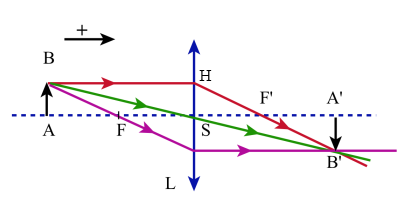
\includegraphics[scale=4]{montageSilberman}\\
		On pose : 
		$$
		\begin{aligned}
		\gamma = \dfrac{\overline{A'B'}}{\overline{AB}} ,\quad y=\overline{AA'},\quad p=\overline{SA},\quad p'=\overline{SA'},\quad \phi=\overline{SF'}=\overline{FS}
		\end{aligned}
		$$
		Montrons que $y=-\phi\dfrac{{(\gamma-1)}^2}{\gamma}$:
		\begin{multicols}{2}
			\begingroup
			\addtolength{\jot}{1em}
			\noindent
			\begin{align*}
			\dfrac{1}{p'}-\dfrac{1}{p}&=\dfrac{1}{\phi} \text{ relation de conjugaison}\\
			\iff p'&=\dfrac{p\phi}{p+\phi}\\
			p'-p &= \dfrac{p\phi}{p+\phi}-p\\
			y &= \dfrac{p\phi-p(p+\phi)}{p+\phi}\\
			y&=-\dfrac{p^2}{p+\phi}
			\end{align*}
			\endgroup
			\setlength\columnseprule{0.4pt}
			\vfill
			\columnbreak
			D'autre part en appliquant le théorème de Thalès aux triangles SHF' et F'A'B':
			\begingroup
			\addtolength{\jot}{1em}
			\noindent
			\begin{align*}
			\gamma&\equiv\dfrac{\overline{A'B'}}{\overline{AB}} = \dfrac{\overline{A'B'}}{\overline{SH}}\\
			&=\dfrac{\overline{A'F'}}{\overline{SF'}}\\
			&=\dfrac{\overline{A'S}+\overline{SF'}}{\overline{SF'}}\\
			&=\dfrac{-p'}{\phi}+1\\
			\iff p' &= -\phi(\gamma-1)
			\end{align*}
			\endgroup
		\end{multicols}
		\vspace*{+1em}
		De plus on sait que : $\dfrac {\overline {AB}} {p}=\dfrac {\overline {A'B'}} {p'}\implies\dfrac{p'}{p}=\gamma$, ainsi :
		\begin{empheq}[left=\empheqlbrace]{align}
		y&=-\dfrac{p^2}{p+\phi}\\
		p' &= -\phi(\gamma-1)\\
		\dfrac{p'}{p}&=\gamma
		\end{empheq}
		En combinant (2) et (3), on obtient : $p=\dfrac{-\phi(\gamma - 1)}{\gamma}$. On injecte dans (1) :
		\begingroup
		\addtolength{\jot}{1em}
		\begin{align*}
		y&=-\dfrac{p^2}{p+\phi}\\
		&=\dfrac{\left( \phi\dfrac{\gamma-1}{\gamma}\right)^2}{\left(\phi\dfrac{\gamma-1}{\gamma}\right) -\dfrac{\phi \gamma}{\gamma}}\\
		&=\dfrac{\phi^2(\gamma-1)^2}{\gamma^2\dfrac{\phi}{\gamma}(\gamma-1-\gamma)}\\
		&=\dfrac{-\phi(\gamma-1)^2}{\gamma}
		\end{align*}
		\endgroup
		On a alors : $y=\dfrac{-\phi(\gamma-1)^2}{\gamma}$\\
		\item 
		Étudions le comportement de la fonction $y(\gamma)$ en supposant $\phi>0$ (lentille convergente). Pour le tracé de la courbe, on pose $\phi=1$, on a alors :
		\begin{figure}[h]
			\centering
			\caption[]{y($\gamma$)}
			\label{fig:graphy}
			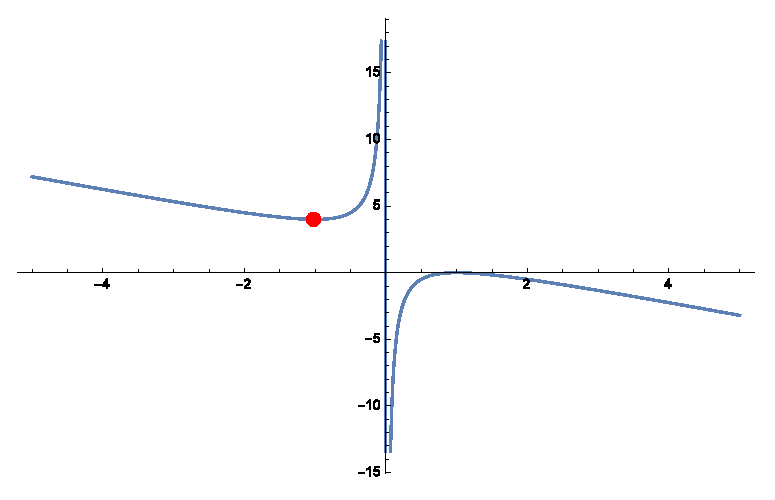
\includegraphics[scale=1.1]{images/GraphY}
		\end{figure}
		La fonction admet un minimum en $\gamma=-1$.\\
		Étudions la fonction plus en détail. On pose $y'\equiv\dfrac {\partial y} {\partial \gamma }$ et $y''\equiv\dfrac {\partial^2 y} {\partial \gamma^2 }$. Montrons que la fonction admet un minimum en -1 :
		\begin{multicols}{2}
			Recherche d'extremum : $y'=0$.\\
			Avec $\phi>0$
			\begin{align*}
			y'&=\left(\frac{1}{\gamma ^2}-1\right) \phi\\
			\end{align*}
			$y'$ s'annule en -1 et 1.
			\setlength\columnseprule{0.4pt}
			\columnbreak
			\\
			Montrons que -1 est un \textsc{Minimum} en étudiant le signe de $y''$:
			\begin{align*}
			y''&=-\dfrac{2}{\gamma^3}\\
			y''(-1)&=2>0
			\end{align*}
		\end{multicols}
		\vspace*{+1em}
		On a $y'(-1)=0 \quad \text{et} \quad y''(-1)>2$, donc -1 est un minimum.\\
		\item Si on se place dans le cas $\gamma=-1$ cela implique $y=4\phi$\\[2pt]
		On en déduit alors : $\phi=\dfrac{y}{4}$
		\item 
		On applique cette méthode sur plusieurs lentilles en prenant en compte une incertitude sur la position de l'écran p' ($\Delta p'=$0,3cm) et une incertitude de lecture sur la position de l'objet p ($\Delta p=$0,3cm).
		$$\phi=\dfrac{y}{4}=\dfrac{p'-p}{4}\implies \Delta \phi = \dfrac{\sqrt{\Delta p^2+\Delta p'^2}}{4}=10^{-1}$$
		\begin{center}
			
			\begin{tabular}{|c|c|c|}
				\hline 
				Lentille n & $\phi_{th}$ (cm) & $\phi_{exp}$ (cm) \\ 
				\hline 
				1 & 12,7 & 12,25$\pm10^{-1}$ \\ 
				\hline 
				2 & 30 & 30$\pm10^{-1}$ \\ 
				\hline 
				3 & 20 & 19,6$\pm10^{-1}$ \\ 
				\hline 
			\end{tabular} 
		\end{center}
		Les valeurs trouvées expérimentalement sont relativement proches de celles inscrites sur les lentilles.
	\end{enumerate}
	\subsection{Méthode de Bessel}
	La méthode de Bessel consiste à fixer l'objet et la position de l'image (i.e l'écran). On déplace la lentille le long de l'axe optique jusqu'à trouver deux positions donnant une image nette.
	\begin{center}
		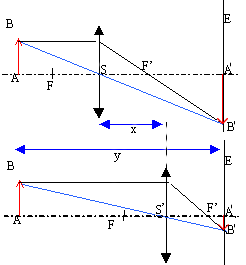
\includegraphics[scale=1]{focale}
	\end{center}
	À partir de la relation de conjugaison, on a déjà montré que si l'on obtient une image réelle d'un objet réel on a : 
	\begin{align*}
	&y=-\dfrac{p^2}{p+\phi}\\
	\iff &p^2 + y.p + y.\phi=0
	\end{align*}
	On cherche des solutions réelles et plus particulièrement le cas où il existe \textsc{deux} solutions réelles. Calculons le discriminant et regardons les conditions pour que $\Delta>0$ ($\implies$ 2 solutions réelles): 
	\begin{align*}
	\Delta &= b^2-4.a.c \\
	&= y^2-4y\phi\\
	&=y(y-4\phi)\\[1em]
	\Delta>0&\implies y>4\phi
	\end{align*}
	Si cette condition est satisfaite, on note $p_+$ et $p_-$ les deux solutions de l'équation :
	$$p_{\pm}=\dfrac{-y\pm\sqrt{y^2-4y\phi}}{2}$$
	On pose $x\equiv p_+ - p_-$ la distance relative entre les deux positions des lentilles (cf. Schéma).
	\begin{align*}
	x&=p_+ - p_-\\
	&=\sqrt{y^2-4y\phi}\\
	\implies x^2 &= y^2-4y\phi\\[1em]
	\iff \phi &= \dfrac{y^2-x^2}{4y}
	\end{align*}
	À partir de ce calcul, on peut dresser un tableau de valeurs:
	\begin{center}
		\begin{tabular}{|c|c|c|c|c|c|c|c|c|c|c|}
			\hline
			i & y & $\Delta y$ & $p_+$ & $\Delta p_+$ & $p_-$ & $\Delta p_-$ & x & $\Delta x$ & $\phi$ & $\Delta\phi$\\
			\hline
			1 & 80,00 & 0,20 & 85,00 & 0,50 & 35,50 & 0,20 & 49,50 & 0,54 & 12,34 & 0,18\\
			\hline
			2 & 140,0 & 0,20 & 63,00 & 0,50 & 17,40 & 0,20 & 45,60 & 0,54 & 31,29 & 0,10\\
			\hline
			3 & 100,0 & 0,20 & 93,50 & 0,50 & 46,50 & 0,20 & 47,00 & 0,54 & 19,48 & 0,14\\
			\hline
		\end{tabular}
	\end{center}
	
	Les résultats expérimentaux sont un peu moins bons que ceux obtenus avec la méthode de Silbermann, mais restent tout de même corrects. Si on calcule l'erreur relative, on trouve que celle-ci est inférieure à 5\% dans chacun des cas.
	\subsection{Commentaires}
	La méthode de Silbermann est un cas particulier de la méthode de Bessel. Selon nous, la méthode de Bessel est plus simple à réaliser, car dans le cas de Silbermann, il faut procéder par tâtonnement en déplaçant la lentille \underline{et} l'écran.
	
	Lorsque l'on s'intéresse aux incertitudes, on constate que la position donnant une image nette n'est pas réellement définie comme un point unique. Les positions $p_+$ et $p_-$ sont sujet à interprétation (généralement de l'ordre du demi-centimètre).\\
	
	Nous cherchons à présent une méthode pour calculer la distance focale d'une lentille convergente. %Nous savons que la puissance résultante de deux lentilles en contact est la somme algébrique de leur puissance. On met donc en contact une lentille convergente de focale connue avec la lentille divergente à déterminer.
	Écrivons les formules de conjugaison des deux lentilles:
	\begin{empheq}[left=\empheqlbrace]{align}
	\dfrac{1}{\overline{S_1A'}} - \dfrac{1}{\overline{S_1A}}=  \dfrac{1}{f_D}\\
	\dfrac{1}{\overline{S_2A''}} - \dfrac{1}{\overline{S_2A'}}=  \dfrac{1}{f_C}
	\end{empheq}
	De plus, on sait que :
	\begin{align}
	\overline{S_2A'} &= \overline{S_2S_1}+\overline{S_1A'} \nonumber \\
	\iff \overline{S_1A'}&=\overline{S_2A'}-\overline{S_2S_1} 
	\end{align}
	On isole $\overline{S_2A'}$ à partir de (5)\\
	\begin{align*}
	\overline{S_2A'}&=\dfrac{\overline{S_2A''}.f_D}{f_D-\overline{S_2A''}}\\[1em]
	\text{(6)}\implies \overline{S_1A'}&=\dfrac{\overline{S_2A''}.f_D}{f_D-\overline{S_2A''}}-\overline{S_2S_1}
	\end{align*}
	Il suffit alors d'isoler $f_D$ dans (4) et de remplacer $\overline{S_1A'}$ par l'expression ci-dessus.
	\begin{multicols}{2}
		\setlength\columnseprule{0.4pt}
		\begingroup
		\addtolength{\jot}{1em}
		\begin{align*}
		f_D&=\dfrac{\overline{S_1A'}.\overline{S_1A}}{\overline{S_1A}-\overline{S_1A'}}\\
		&=\dfrac{-10.-46}{-46+10}\\
		&=12,8\pm0,38\text{ cm}
		\end{align*}
		\vfill
		\columnbreak
		\begin{align*}
		\overline{S_1A'}&=\dfrac{\overline{S_2A''}.f_D}{f_D-\overline{S_2A''}}-\overline{S_2S_1}\\
		&=\dfrac{60.20}{20-60}+20\\
		&=-10\pm0,25\text{ cm}
		\end{align*}
		\endgroup
	\end{multicols}
	
	\begin{figure}[h]
		% \centering
		\begin{bigcenter}
			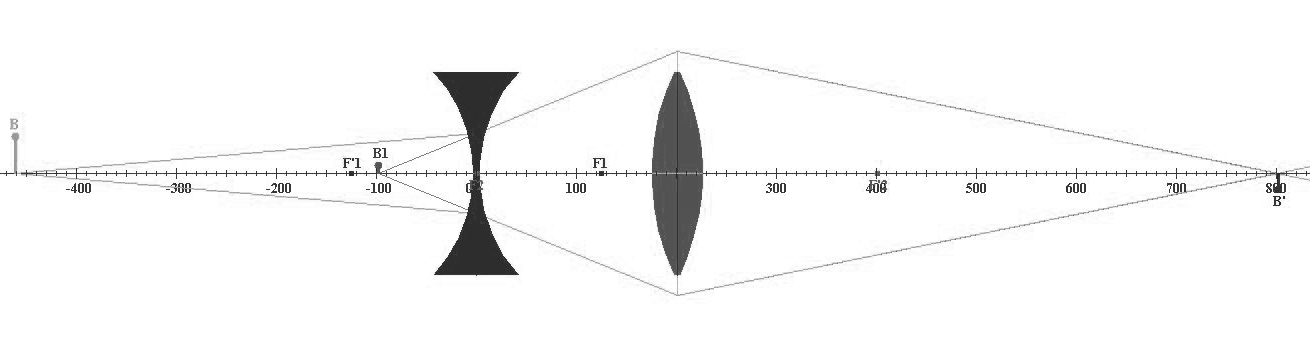
\includegraphics[scale=0.7]{images/divergente}
			\caption[]{Montage de détermination de la focale d'une lentille divergente}
			\label{fig:divergente}
		\end{bigcenter}
	\end{figure}
	
	Compte tenu des incertitudes, la valeur théorique correspond à la valeur indiquée sur la lentille.
	\section{Aberrations}
	L'étude des aberrations s'effectue en utilisant des lentilles convergentes ayant une courbure importante
	\subsection{Aberration sphérique}
	On propose une étude qualitative de cette aberration géométrique en effectuant un relevé de points mettant en évidence l'existence de la caustique. On étudie la nappe tangentielle en relevant le diamètre de l'image en fonction de l'éloignement de l'écran.
	\begin{center}
		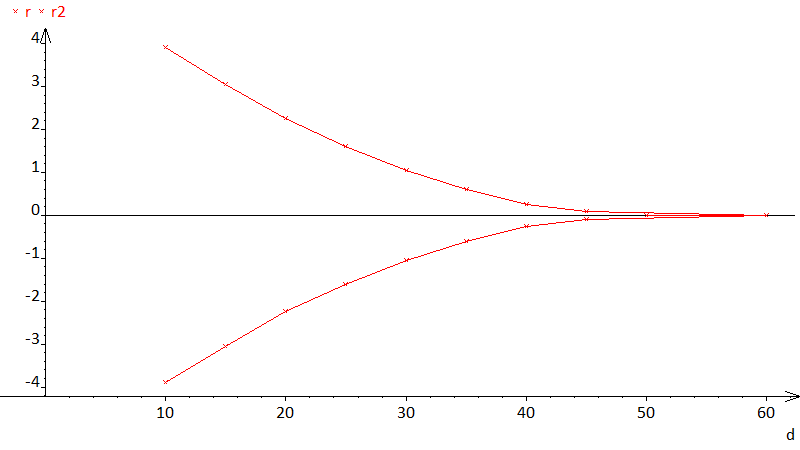
\includegraphics[scale=0.5]{images/caustique}
	\end{center}
	On trouve une forme se rapprochant de la forme caractéristique de l'aberration sphérique.
	\subsection{Aberration chromatique}
	Pour pouvoir observer le phénomène d'aberration chromatique, on cherche à faire l'image d'un trou à travers une lentille convergente. On fixe l'objet et la lentille et on déplace l'écran le long de l'axe optique jusqu'à trouver le foyer. C'est alors que l'on met en évidence l'aberration chromatique puisqu'il n'existe plus un foyer unique. On distingue très clairement dans notre cas un foyer bleu puis un foyer rouge plus éloigné de la lentille. Ce phénomène s'explique, car la courbure de la lentille est telle que l'on peut l'assimiler à un prisme pour les rayons les plus éloignés de l'axe optique.
	
	On nous a donné $n=A+\dfrac{B}{\lambda^2}\implies$l'indice dépend de la longueur d'onde et les petites longueurs d'onde sont plus déviées (milieu plus réfringent au petit n). Or on sait que :
	\begin{align*}
	\lambda_{bleu}(\approx400nm)&<\lambda_{rouge}(\approx800nm)\\
	\implies n_{bleu}&>n_{rouge}
	\end{align*}
	Il est donc normal que le bleu converge plus et que son foyer soit situé avant celui du rouge.
\end{document}